\chapter{Coding}
\label{chap:Coding}



\begin{rem}
Use meaningful names. Refrain from 
using \code{v}, then double v; \code{vv},
and then \code{w}.
\end{rem}


\begin{rem}
Refrain from copying your code from
one file to another.
\end{rem}
\noindent When you copy your code from one file/module
to another, it means you use it a lot. Thus, you can
save it in a unique module and call it again and again.
This is easier, faster, and more importantly sustainable.
For example, if you plot a vector with your favorite settings,
write a function once then use it. If later you need
to change the font to be consistent with
the journal you want to submit your paper to, then, you can
change the font only once. Otherwise, you have to go to
all the files you wrote before and change them one at a time!
Just stop copy/pasting.

In~\cref{fig:FunctionDocumentation} we see how a function is defined
and documented in Python.
A few points to make here using this example are given below.
\begin{figure}
  \centering
  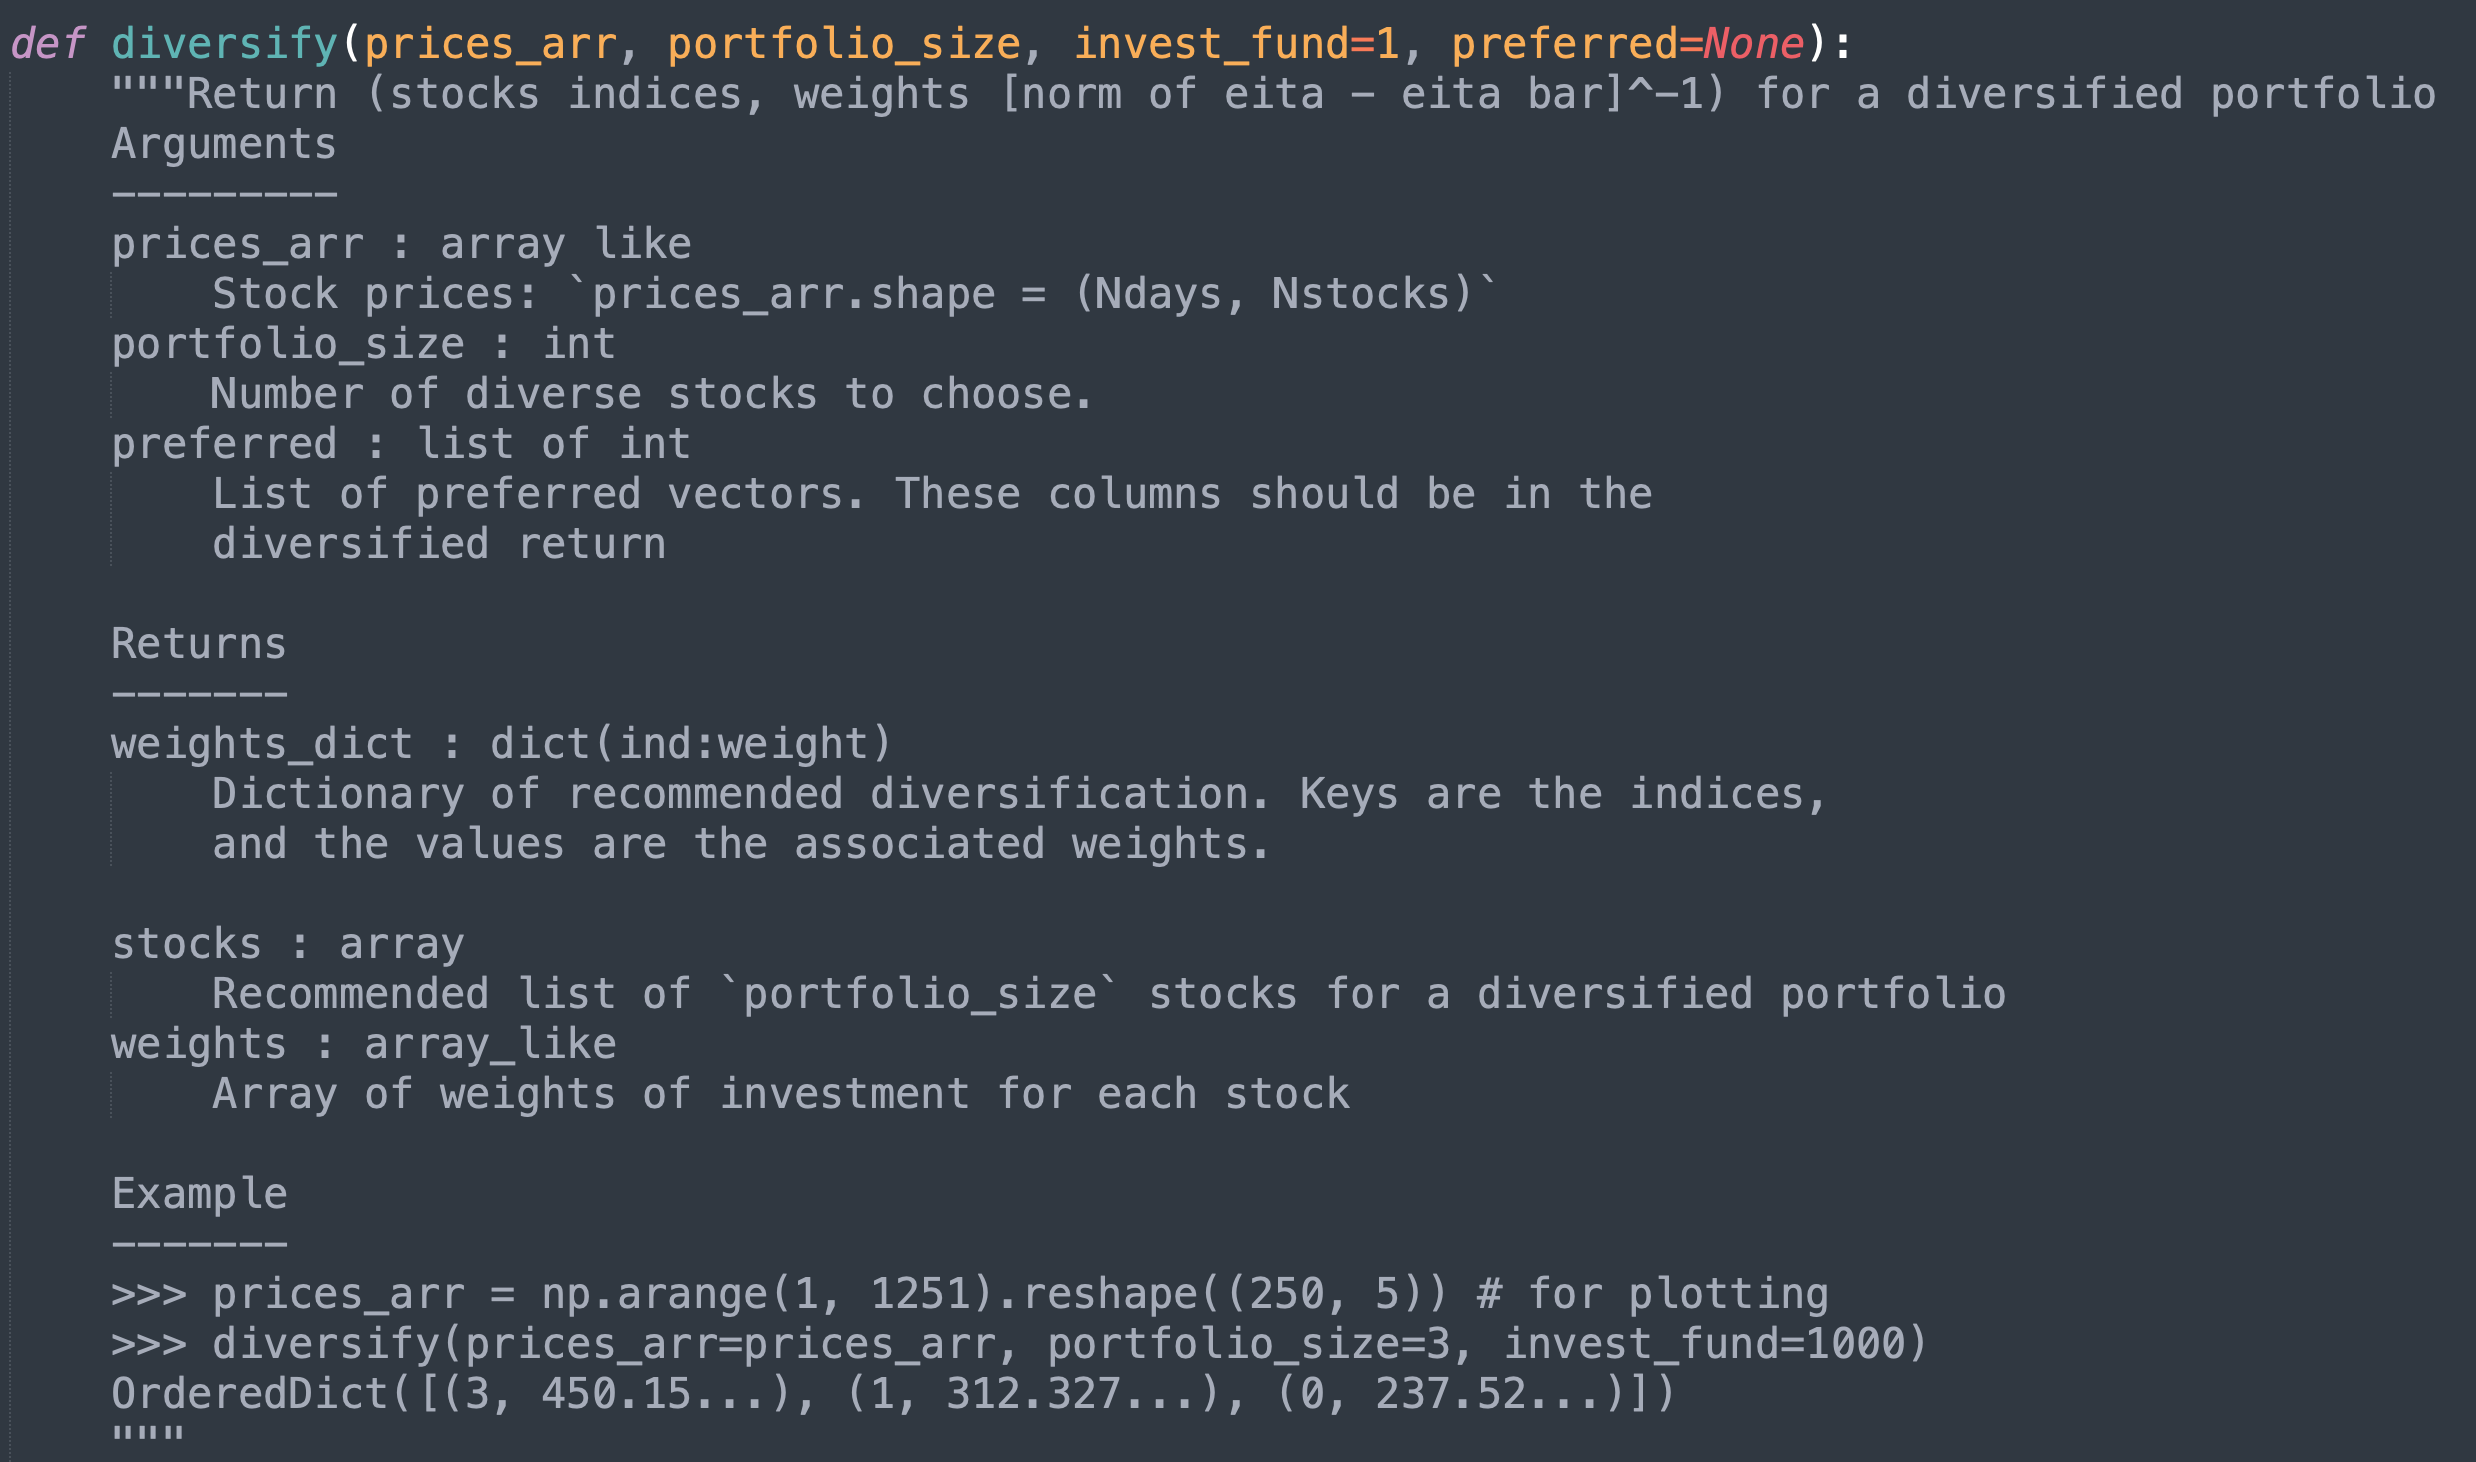
\includegraphics[width=1\textwidth]{figures/function_documentation}
  \caption{Function Documentation.}
  \label{fig:FunctionDocumentation}
\end{figure}

\noindent Remarks about the function in~\cref{fig:FunctionDocumentation};
\begin{description}
\item [Function Name] is meaningful.
\item [Input Variables] have meaningful name. 
\item [First Input Variable] There are different conventions. In this
example we see the first input variable is named \code{prices\_arr}.
We see that not only the variable name is meaningful but also
it is implying the type of the variable. It is an array. It is not a list.
It is not a panda dataframe. 

\item [Variables with Default values] come last.

\item [Function's Description] Include the functions' descriptions
the first thing in the function. The first line (text) can describe what the function does. 
Then, define the arguments; input variables. 
We have \code{prices\_arr : array like} and then in the line below \code{Stock prices: `prices\_arr.shape = (Ndays, Nstocks)'}.
So, immediately after the variable name its type is specified. In the line that follows we
say what it is representing.

\item [Include Example(s)] You can include an example at the end of the
description to show how the function is used. This is not necessary unless
later you want to share your code, form a library and release it.
Then, you can have pages
like Python's documentation pages.

\item [Make Comments] throughout the code and functions.
Write down what each line is doing or why. You can skip
simple stuff. If you do not make comments and need to use
the code after a month you may have hard time remembering.
\end{description}
The example above is on \href{https://github.com/HNoorazar/Ag/blob/master/Kirtis\_Class/Python/Kirtis\_Class\_core.py}{GitHub} for you to review.
The convention used for documentation is the same as 
that of numpy~\citep{numpyStyle}.

Once you write your functions in a central module
you can import them into your driver modules and use
them the way you import standard libraries/packages of Python or R.

Say we have two modules that are the engine of our project.
\marginnote{I use sublime text editor to write my codes}
One includes all the functions that generate stuff and the other
includes all the plotting functions; \code{kirtis\_class\_core.py},
\code{kirtis\_class\_plot\_core.py}.
Say these two modules are saved in 
the following directory:
\code{/Users/Documents/project1/}.
Then we can import these modules into our driver
and use them like so:

\begin{tcolorbox}
  \begin{algorithm}[H]
  \label{alg:importPythonCode}
   \caption{Import Your Python Modules.}
\SetAlgoLined
0. \codeGreen{import} \code{sys}\;
1. \code{sys.path.append(}'\codeRed{/Users/Documents/project1/}'\code{)}\;
2. \codeGreen{import} \code{kirtis\_class\_core} \codeGreen{as} \code{kcc} \;
3. \codeGreen{import} \code{kirtis\_class\_plot\_core} \codeGreen{as} \code{kcpc} \;
4.Use the function \codeCyan{diversify} from \code{kirtis\_class\_core.py} like \\
\code{diversified\_portfolio = kcc.\codeCyan{diversify}(\codeGoldenrod{x}, \codeGoldenrod{y}, \codeGoldenrod{z})}
\end{algorithm}
\end{tcolorbox}
A simple code demonstrating this is on GitHub that you can look at;
\href{https://github.com/HNoorazar/Ag/tree/master/Kirtis\_Class/Python}{github.com/HNoorazar/Ag/tree/master/Kirtis\_Class/Python}.\\

In a similar way you can import your R modules into the drivers.
Say your R module with all the functions in it is called \code{R\_engine\_core.R}
located in \code{/Users/Documents/project1/}.
You can import it like so in your driver:

\begin{tcolorbox}
  \begin{algorithm}[H]
  \label{alg:importRCode}
   \caption{Import Your R Modules.}
\SetAlgoLined
1. \code{source\_path =} \codeGreen{"Users/Documents/project1/R\_engine\_core.R"} \;
2. \code{source(source\_path)} \;
3.Use the function \codeCyan{diversify} from \code{R\_engine\_core.R} like you use any function of R: \\
\code{diversified\_portfolio = \codeCyan{diversify}(\codeGoldenrod{x}, \codeGoldenrod{y}, \codeGoldenrod{z})}
\end{algorithm}
\end{tcolorbox}








